%
%                       This is a basic LaTeX Template
%                       for the Informatics Research Review

\documentclass[a4paper,11pt]{article}
% Add local fullpage and head macros
\usepackage{head,fullpage}     
% Add graphicx package with pdf flag (must use pdflatex)
\usepackage[pdftex]{graphicx}  
% Better support for URLs
\usepackage{url}
% Date formating
\usepackage{datetime}
% For Gantt chart
\usepackage{pgfgantt}
\usepackage{xcolor}
\usepackage[utf8]{inputenc}
\usepackage{tabularx}
\newdateformat{monthyeardate}{%
  \monthname[\THEMONTH] \THEYEAR}

\parindent=0pt          %  Switch off indent of paragraphs 
\parskip=5pt            %  Put 5pt between each paragraph  
\Urlmuskip=0mu plus 1mu %  Better line breaks for URLs


%                       This section generates a title page
%                       Edit only the following three lines
%                       providing your exam number, 
%                       the general field of study you are considering
%                       for your review, and name of IRR tutor

\newcommand{\examnumber}{B208489}
\newcommand{\field}{Agent-based Modelling}
\newcommand{\tutor}{Valentina Andries}
\newcommand{\supervisor}{Valerio Restocchi}

\begin{document}
\begin{minipage}[b]{110mm}
        {\Huge\bf School of Informatics
        \vspace*{17mm}}
\end{minipage}
\hfill
\begin{minipage}[t]{40mm}               
        \makebox[40mm]{
        
\includegraphics[width=40mm]{diagrams/crest.png}}
\end{minipage}
\par\noindent
    % Centre Title, and name
\vspace*{2cm}
\begin{center}
        \Large\bf Agent-based modelling for sustainable banking  \\
         \Large\bf --- collaboration with ekko\\
        \Large\bf \field
\end{center}
\vspace*{1.5cm}
\begin{center}
        \bf \examnumber\\
        \monthyeardate\today
\end{center}
\vspace*{5mm}

%
%                       Insert your abstract HERE
%                       
\begin{abstract}
        Ecosystems are under threat from climate change. However, the link between reducing carbon emissions and spending behaviour exists, and the project aims to use the link to reduce the individual carbon footprint.
The project uses an agent-based modelling approach to analyse people spending habits and discovers new influence maximisation strategies to encourage people to purchase at sustainable companies.
\end{abstract}

\vspace*{1cm}

\vspace*{3cm}
Date: \today

\vfill
{\bf Tutor:} \tutor\\
{\bf Supervisor:} \supervisor
\newpage

%                                               Through page and setup 
%                                               fancy headings
\setcounter{page}{1}                            % Set page number to 1
\footruleheight{1pt}
\headruleheight{1pt}
\lfoot{\small School of Informatics}
\lhead{Informatics Research Review}
\rhead{- \thepage}
\cfoot{}
\rfoot{Date: \date{\today}}
%


\section{Motivation}

Nowadays, our attention to environmental issues has been increasing, and the environmental issues we face are getting more and more severe. One way that everyone can contribute to environmental protection in our daily life is to reduce their carbon footprint, which is the total amount of greenhouse gases caused by our actions \cite{3}. When we buy different products in different places, greenhouse gas emissions also vary, but we can find a method to encourage people to buy products at sustainable companies \cite{4}. Hence, we need to understand people spending habits and how to make valid influences.
Agent-based modelling (ABM) is a simulation technique that captures individual behaviour in an environment that has been applied to many real-world problems in recent years, especially for business problems \cite{1}.
Most business problems are hard to simulate as we do not know the behaviour of the system or the system is too complex for conventional approaches. However, the ABM provides a way to simulate a large number of decisions by individual entities with simple decision rules \cite{5}. 
If we successfully simulate the business problem, we could understand the inner logic of the system, how individual entities act and interact with each other and the market or even discover the reason that might cause business failure.
Moreover, we can also change the rules of the ABM and observe the reflection of the model before we apply changes to the real-world problem to avoid loss.
Therefore, in this project, we will focus on the spending habit of people. We aim to build an ABM that successfully simulates people's daily spending habits and find new influence maximisation strategies that affect people's spending habits based on the ABM. Then we could apply the influence strategies to encourage people to reduce their carbon footprint.


\subsection{Feasibility}
This is an industry-supported project, so the transaction data will be provided by ekko as spending habit data. We could use network science to analyse the behaviour of user groups and use the obtained information to build and test the ABM. Then, we could start to find influence maximisation strategies with our ABM.

\subsection{Beneficiaries}

With the actual data analysis and ABM model results, we could apply the strategies to the real world to encourage people to shop at greener companies. In addition, we could use our user spending habits results to help the industry provide more satisfying services for customers.

\section{Background and Related Work}
\subsection{Network Science}
Networks appear in all kinds of aspects of our life, so it becomes a powerful way to represent and analyse complex interactions \cite{6}. A network can be treated as a graph where nodes can represent different individuals, and links represent interactions between them. According to the described system situation, the network can be classified into weighted or unweighted, and directed or undirected \cite{7}. We could obtain a conceptional understanding of the system by analysing the network model, hub, community, and pattern.

\subsection{Agent-based Modeling}
The ABM provide a bottom-up way of describing the system and is a microscale model. In agent-based modelling, a system is built by autonomous agents. Each agent in this system has to make decisions based on a set of rules, and agents behave differently to represent different systems \cite{3}.
Therefore, the ABM aims to use multiply agents to reproduce or predict a complex phenomenon as the ABM simulates all agents' interactions simultaneously and also captures emergent phenomena \cite{2}. 
The result of the ABM has high randomness and is hard to predict as we can only set the rules and agents' behaviour at the beginning, and we can not control the growth of the model.
Hence, it is an excellent way to test our understanding of the system.

\subsection{Related Work}
Using an agent-based modelling approach to simulate a human involved system and analysis the human spending habits is not rare. For example, Andrea et al. provide an agent-based modelling simulation of customer behaviour in meat consumption in Britain with consideration of individual preferences and peer influence \cite{ABM_meat}. 
Agents are created with different gender, ages, salary, employment status, diet, and others. Each agent has a meat consumption probability that is updated with time (every meal) according to the agent's socio-demographic characteristics, individual concerns, influence from other agents, and meat price.
Agents in the same family can influence each other, and co-workers can be influenced through the workplace network \cite{ABM_meat}.
This ABM approach to customer behaviour in meat consumption provides an idea to implement our ABM model. We could use a similar method to define our agents and market, extending from the demand for meat to the demand for other daily necessities to capture customers' spending habits.
Aurelija et al. also conduct an ABM framework to investigate the customer behaviour in the insurance field that we can learn from the model implementation procedure \cite{ABM_insu}.

Moreover, David Andersson developed an application to calculate the individual carbon footprint from the financial transaction data \cite{cb_app}. It used a novel hybrid approach to estimate the carbon footprint of users with three data sources shown in figure \ref{cb_app_source}. All transaction data are classified based on the Classification of Individual Consumption According to Purpose (COICOP), so the application could estimate GHG emissions according to different consumption categories of transactions \cite{cb_app}. 

In terms of agent-based modelling with influence strategies, Haer et al. present an example with an agent-based model to analyse flood risk communication strategies \cite{ABM_flood}. The paper analyses the effect on individuals with different flood risk communication strategies and the role of social networks in this process. The ABM model uses four different flood risk communication strategies compared to a baseline scenario with different probability and stander deviation to change agents' attitudes toward the flood risk \cite{ABM_flood}. Hence, we could use a similar approach to evaluate the most effective strategy that affects individual spending habits on greener companies.

By combining the related research above, we could have a clearer understanding of approaching the project step by step.


\begin{figure}
    \centering
    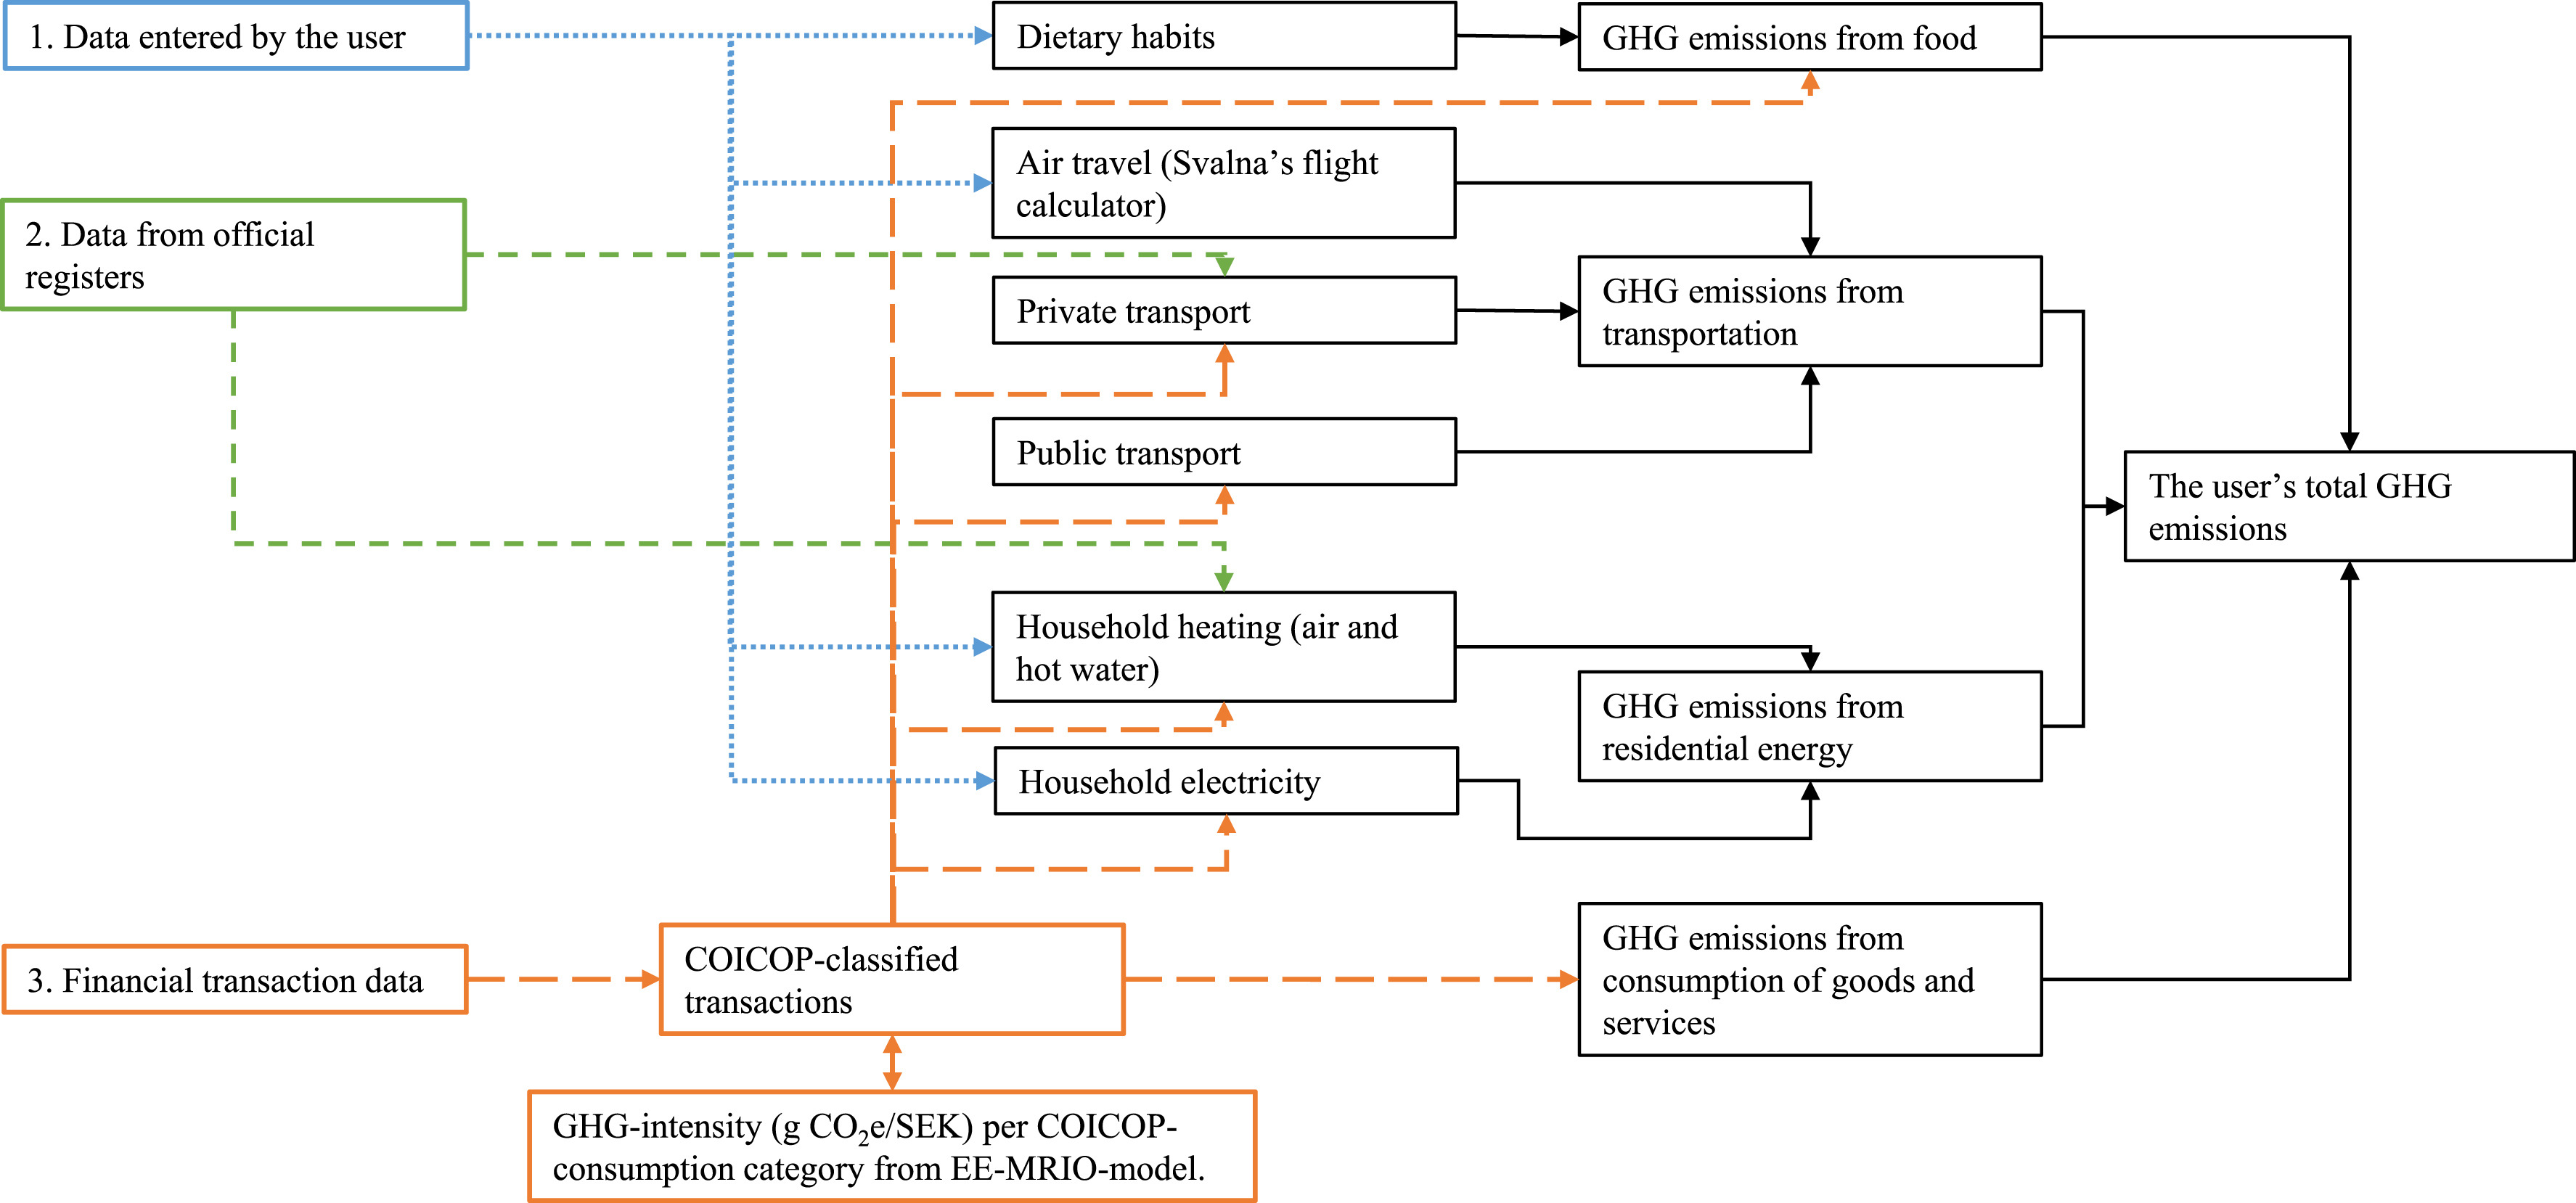
\includegraphics[width=\linewidth]{diagrams/cb_app_source}
    \caption{Schematic overview of various sources in order to estimate GHG emissions at the individual level}
    \label{cb_app_source}
\end{figure}

\section{Programme and Methodology}

\subsection{Transaction Data}
Bank transaction data are provided by ekko and are expected to contain basic payment information shown in table \ref{bank_data}.
attributes of bank transaction data
We also expected to have basic user information, including gender, year of birth, home location, average salary and other information that could help with analysis.
\begin{table}[htbp]
    \begin{center}
        \begin{tabular}{|c|l|}
        \hline
        \textbf{Attribute} & \textbf{Description} \\
        \hline
        tran\_ID & transaction ID\\
        user\_ID & user ID \\\
        acc\_num & account number \\
        tran\_tp & transaction type (eg. credit, debit) \\
        tran\_date & transaction date \\
        tran\_cat & category of the transaction provided by bank (eg. supermarket, restaurant)\\
        tran\_amt & amount of money of the transaction \\
        \hline
        \end{tabular} 
    \end{center}
    \caption{Attributes of Bank Transaction Data}
    \label{bank_data}
\end{table}

\subsection{Data analysis}
After obtaining and organising the project data, we could start data analysis using network science. 
To adjust and refine the ABM model, we need to find the pattern of the user groups and transaction data as the actual value.
Moreover, we would like to identify the factors that affect spending habits with the user information. 
For example, place of residence has a substantial impact on people's spending habits based on exploring the individual economic behaviour \cite{city_bx}.
We could classify the users into different groups according to the factors we discovered, and groups can overlap. In addition, spending behaviour can also be characterised from the bank transaction data such as overall spending behaviour, temporal spending behaviour \cite{psy_bx}.
According to the classified user groups and characterised spending behaviour, we could draw a user sample model representing our unbiased ABM human agents. In the user sample model, each user has one or two characterised spending behaviour and several classified factor groups.

\subsection{Model creation and evaluation}
To build the ABM, we could reproduce the user sample model we analysed as human agents and form appropriate rules according to their characteristics. 
The update of the agent status is expected to be daily, and we could observe the result of agents' behaviour at daily intervals.
The environment of the ABM should simulate the real-world market, which reflects the amount of carbon emission and commodity price. Different data sources can be used to modify the market and carbon emission, and multiple aspects can influence the real-world market. Thus, we could find a suitable market data combination according to the data pattern we obtained from the analysis.
Validation of the ABM model is also based on the information we analysed from the actual data to confirm that we successfully simulated the user spending habits. Then, we could apply sensitivity analysis to analyse the model behaviour and output to ensure the model is valid.

\subsection{Influence Strategy and Carbon Footprint Reduction}
An influence strategy must be a reasonable strategy that can be applied to the real world and is worth comparing to the disburse. Therefore, we have to collaborate with ekko to discuss a couple of practical influence strategies. If available, we could also get some feedback or data on these influence strategies to help us apply the influence strategies to the ABM. Otherwise, we could make assumptions with ekko combining similar influence strategies results from other experiments to apply the strategies.
There are also some network influence models that can be considered to model how information spreads through agents, such as the independent cascade model \cite{7}.
Marten's paper presents a method from a new perspective to target customers using the pseudo-social network that links the customers that transfer money to the same entities \cite{psn}.
According to the results of different influence strategies we applied to the ABM, we could uncover the influence strategy or influence strategy combination with the best performance that encourages people to reduce their daily carbon footprint.

\subsection{Risk Assessment}
This project is more practical than theoretical, so there will be many unforeseen problems.
As we can not obtain the data until the start of the program, there is the probability that the data is not what we expected or not available. Moreover, we do not know the selection procedure of the data yet. Although we assume that the users and their transaction data are selected randomly, bias might be involved. 
We do not know whether ekko will provide their carbon footprint calculation method, so we assume we would use transaction data to estimate the carbon footprint. Besides the main risks mentioned above, other risks are listed in table \ref{risk_table}.

\begin{table*}[htbp]
    \begin{center}
        \begin{tabularx}{\textwidth}{|p{4cm}|c|c|X|}
        \hline
        \textbf{Risk} & \textbf{Probability}  & \textbf{Severity}  & \textbf{Actions to Minimise Risk} \\
        \hline
        Cannot get transaction data & Very unlikely & Severe & Find other available data sources as soon as possible \\
        \hline
Cannot get transaction data on time & Unlikely & Moderate & Keep communication with ekko, ensure the latest time for the data and start the reading part of the project first \\
\hline
Cannot get user information & Likely & Moderate & Estimate the user group data with the open data source (e.g. Worldbank Database) \\
\hline
Data selection is biased & Likely & Minor & Although it would affect the analysis result, the ABM is also built with the biased data. Hence, the influence strategy is still suitable for the original users provided, and we would identify bias in the final report \\
\hline
No significant pattern while analysing transaction data & Likely & Minor & Try to identity hubs, community and any outlier that affect the result, combine the information we have to describe the data structure \\
\hline
Too much data to process & Unlikely & Not Significant & Separate the data according to month, weeks or day to analysis in time series, or separate the data according to user group \\
\hline
No significant spending behaviour difference & Unlikely & Minor & Simplify the characterised spending behaviour section \\
\hline
Cannot build a valid ABM simulate the given data & Unlikely & Severe & Revise the procedure of building the ABM, find out the possible problem, keep communication with supervisor to ensure the project is in the right direction \\
\hline
Cannot have influence strategies data & Likely & Minor & We could make assumptions and use similar experiment data. However, the accuracy of the result would be affected if applied to the actual situation \\
\hline
Leak user data & Very Unlikely & Severe & Find data leakage channels and stop losses in time. Try to keep the data locally without uploading it to other platforms, use a self-owned computer to complete projects and keep the computer safe \\
        \hline
        \end{tabularx} 
    \end{center}
    \caption{Risk Assignment Table}
    \label{risk_table}
\end{table*}

\subsection{Ethics}
The project will abide by the ethical standards of the University of Edinburgh throughout.
Although we would deal with the real user transaction data, we do not collect the data personally and have contact with any user. Thus, we do not need to apply for ethical approval for the project. Indeed, we still need to ensure user data security and prevent user information leaks mentioned in the risk assessment section.

\section{Evaluation}

The project data is provided by ekko, so we do not have problems related to data collection. To ensure the ABM built is valid, we would conduct the model validation using analysed results and sensitivity analysis mentioned in the model evaluation section. Influence strategy selection is based on the result of influence on the valid ABM model. Although we might need to make some assumptions about the impact of the strategies, the assumptions would be made based on experiments and data analysis. We would run validation tests or prove with data on the assumptions created.
Thus, the influence strategies selected are valid and unbiased if the original data provided is unbiased.

\section{Expected Outcomes}

To conclude, the project would present an agent-based model that simulates the user spending behaviour analysed from the transaction data provided by ekko. Moreover, we would find out the influence strategies that maximise the influence on encouraging users to purchase at sustainable companies.
This project will deliver a different point of view in the analysis of daily spending behaviour as it uses the ABM approach, which is not common. Moreover, our ecosystem is threatened by the climate change problem, and each individual needs to take responsibility. The project could be the bond between reducing carbon emissions and daily life. Although this project might be less helpful in filling theoretical gaps, it is practical and can be put on the market after certain considerations.


\section{Research Plan, Milestones and Deliverables}

The project can be divided into three stages: preparation, implementation and documentation, and the implementation of the project is split into four parts. The Gantt chart demonstrates the project plan shown in figure \ref{gantt_c}.
The black lines in the Gantt chart indicate the expected time for the stage, and the blue bar indicates the time predicted for each part of the stage.
The black lines are slightly longer than the blue bars in each stage as we set aside time to deal with unexpected situations.
The first stage is the preparation which we wait for the industry data and complete the related reading. The data is expected to be delivered in early June, so we expect to finish the reading while waiting for the data and organise the data by the middle of June. 
We could start the data analysis process once the data is organised, and we expected to spend eight to ten days for each part in the implementation stage. Data analysis and model evaluation might take less time than others, and influence strategy might need to communicate with ekko, which increases the estimated time. The planned time is relatively generous to ensure each part can be completed on time.
There are two documents that need to be delivered during the project procedure. Project progress is required in week 6 with a short length so that we could plan less time on it. The dissertation is the most crucial part of the project with a heavy workload. Therefore, we could start writing along with the project progress and refine the dissertation after project implementation is completed.
Milestones are listed in table \ref{stone} with a two-week interval to ensure the stability of the project schedule. Deliverables are listed in table \ref{del} according to the milestones.

\definecolor{barblue}{RGB}{0, 153, 153}
\definecolor{groupblue}{RGB}{249,176,29}
\definecolor{linkred}{RGB}{165,0,33} 
\definecolor{bg}{RGB}{0,204,204} 

\begin{figure}[htbp]
\begin{ganttchart}[
    y unit title=0.4cm,
    y unit chart=0.5cm,
    vgrid,hgrid,
    x unit=1.55mm,
    time slot format=isodate,
    title/.append style={draw=none, fill=barblue},
    title label font=\sffamily\bfseries\color{white},
    title label node/.append style={below=-1.6ex},
    title left shift=.05,
    title right shift=-.05,
    title height=1,
    bar/.append style={draw=none, fill=groupblue},
    bar height=.6,
    bar label font=\normalsize\color{black!50},
    group right shift=0,
    group top shift=.6,
    group height=.3,
    group peaks height=.2,
    bar incomplete/.append style={fill=bg}
   ]{2022-06-01}{2022-08-20}
   \gantttitlecalendar{month=name}\\
   
   \ganttbar[
    progress=100,
    bar progress label font=\small\color{barblue},
    bar progress label node/.append style={right=4pt},
    bar label font=\normalsize\color{barblue},
    name=pp
   ]{Project proposal }{2022-06-01}{2022-06-1} \\
   
\ganttset{progress label text={}, link/.style={black, -to}}
\ganttgroup{Preparation}{2022-06-2}{2022-06-15} \\
\ganttbar[progress=50, name=T1A]{Background Reading}{2022-06-2}{2022-06-10} \\
\ganttbar[progress=0]{Data Organisation}{2022-06-2}{2022-06-10} \\

\ganttgroup{Implementation}{2022-06-16}{2022-07-30} \\
\ganttbar[progress=0, name=T2A]{Data Analysis}{2022-06-16}{2022-06-24} \\
\ganttlinkedbar[progress=0]{Model Creation}{2022-06-24}{2022-07-4} \\
\ganttlinkedbar[progress=0]{Model Evaluation}{2022-07-04}{2022-07-12} \\
\ganttlinkedbar[progress=0]{Influence Strategy}{2022-07-12}{2022-07-22} \\


\ganttgroup{Documentation}{2022-06-2}{2022-08-19} \\
  \ganttbar[progress=0]{Progress Report}{2022-07-10}{2022-07-15}\\
   \ganttbar[progress=0]{Dissertation}{2022-06-2}{2022-08-15}
  \ganttset{link/.style={green}}
  \ganttlink[link mid=.4]{pp}{T1A}
  \ganttlink[link mid=.159]{pp}{T2A}
\end{ganttchart}
\caption{Gantt Chart of the activities defined for this project.}
\label{gantt_c}
\end{figure}

\begin{table}[htbp]
    \begin{center}
        \begin{tabular}{|c|c|l|}
        \hline
        \textbf{Milestone} & \textbf{Week} & \textbf{Description} \\
        \hline
        $M_1$ & 2 & Preparation completed \\
        $M_2$ & 4 & Data analysis completed \\
        $M_3$ & 6 & Model creation completed \\
        $M_4$ & 7 & Model evaluation completed \\
        $M_5$ & 8 & Project implementation completed \\
        $M_6$ & 10 & Submission of dissertation \\
        \hline
        \end{tabular} 
    \end{center}
    \caption{Milestones defined in this project.}
    \label{stones}
\end{table}

\begin{table}[htbp]
    \begin{center}
        \begin{tabular}{|c|c|l|}
        \hline
        \textbf{Deliverable} & \textbf{Week} & \textbf{Description} \\
        \hline
        $D_1$ & 4 & Data analysis result\\
        $D_2$ & 6 & ABM model\\
        $D_3$ & 6 & Progress report \\
        $D_4$ & 8 & Influence Strategies \\
        $D_5$ & 10 & Dissertation \\
        \hline
        \end{tabular} 
    \end{center}
    \caption{List of deliverables defined in this project.}
    \label{del}
\end{table}


\begin{thebibliography}{9}
\bibitem{3}
Footprintnetwork.org. 2022. Climate Change \& the Carbon Footprint. [online] Available at: <https://www.footprintnetwork.org/our-work/climate-change/> [Accessed 27 April 2022].
\bibitem{4}
Selin, N., 2020. carbon footprint | Definition, Examples, Calculation, Effects, \& Facts. [online] Encyclopedia Britannica. Available at: <https://www.britannica.com/science/carbon-footprint> [Accessed 27 April 2022].
\bibitem{1}
Bonabeau, E., 2002. Agent-based modeling: Methods and techniques for simulating human systems. [online] Available at: <https://www.pnas.org/doi/10.1073/pnas.082080899> [Accessed 27 April 2022].
\bibitem{5}
North, M. and Macal, C., 2007. Managing business complexity : b discovering strategic solutions with agent-based modeling and simulation. Oxford: Oxford University Press, p.328.
\bibitem{6}
Barabási, A., 2013. Network science. Philosophical Transactions of the Royal Society A: Mathematical, Physical and Engineering Sciences, 371(1987), p.20120375.
\bibitem{7}
Menczer, F., Fortunato, S. and Davis, C., 2020. A First course in network science. Cambridge [etc.]: Cambridge University Press.
\bibitem{2}
Rand, W. and Rust, R., 2011. Agent-based modeling in marketing: Guidelines for rigor. International Journal of Research in Marketing, 28(3), pp.181-193.
\bibitem{ABM_meat}
Scalco, A., Macdiarmid, J., Craig, T., Whybrow, S. and Horgan, G., 2019. An Agent-Based Model to Simulate Meat Consumption Behaviour of Consumers in Britain. Journal of Artificial Societies and Social Simulation, 22(4).
\bibitem{ABM_insu}
Ulbinaitė, A. and Moullec, Y., 2010. TOWARDS AN ABM-BASED FRAMEWORK FOR INVESTIGATING CONSUMER BEHAVIOUR IN THE INSURANCE INDUSTRY. Ekonomika, 89(2), pp.95-110.
\bibitem{cb_app}
Andersson, D., 2020. A novel approach to calculate individuals’ carbon footprints using financial transaction data – App development and design. Journal of Cleaner Production, 256, p.120396.
\bibitem{ABM_flood}
Haer, T., Botzen, W. and Aerts, J., 2016. The effectiveness of flood risk communication strategies and the influence of social networks—Insights from an agent-based model. Environmental Science \&amp; Policy, 60, pp.44-52.
\bibitem{city_bx}
Sobolevsky, S., Sitko, I., Tachet des Combes, R., Hawelka, B., Murillo Arias, J. and Ratti, C., 2016. Cities through the Prism of People’s Spending Behavior. PLOS ONE, 11(2), p.e0146291.
\bibitem{psy_bx}
Tovanich, N., Centellegher, S., Bennacer Seghouani, N., Gladstone, J., Matz, S. and Lepri, B., 2021. Inferring psychological traits from spending categories and dynamic consumption patterns. EPJ Data Science, 10(1).
\bibitem{psn}
Martens, David and Provost, Foster, Pseudo-Social Network Targeting from Consumer Transaction Data (September 2011). NYU Working Paper No. CEDER-11-05, Available at SSRN: https://ssrn.com/abstract=1934670
\iffalse
\bibitem{ABM_human}
Bonabeau, E., 2002. Agent-based modeling: Methods and techniques for simulating human systems. Proceedings of the National Academy of Sciences, 99(suppl\_3), pp.7280-7287.
\bibitem{ABM_simu}
Macal, C. and North, M., 2005. Tutorial on agent-based modeling and simulation. Proceedings of the Winter Simulation Conference, 2005., pp. 14 pp.-.
\fi
\end{thebibliography}
\end{document}

